

%----------------------------------------------------------------------------------------
%	PACKAGES AND DOCUMENT CONFIGURATIONS
%----------------------------------------------------------------------------------------

\documentclass{article}
\usepackage[margin=1in]{geometry}
\usepackage[version=3]{mhchem} % Package for chemical equation typesetting
\usepackage{siunitx} % Provides the \SI{}{} and \si{} command for typesetting SI units
\usepackage{graphicx} % Required for the inclusion of images
\usepackage{natbib} % Required to change bibliography style to APA
\usepackage{amsmath} % Required for some math elements 

\setlength\parindent{0pt} % Removes all indentation from paragraphs

\renewcommand{\labelenumi}{\alph{enumi}.} % Make numbering in the enumerate environment by letter rather than number (e.g. section 6)

%\usepackage{times} % Uncomment to use the Times New Roman font

%----------------------------------------------------------------------------------------
%	DOCUMENT INFORMATION
%----------------------------------------------------------------------------------------

\title{Lab Report of Laser Spectroscopy \\ Demonstration of ns-Laser Flash photolysis Setup} % Title

\author{Tao \textsc{Li}} % Author name

\date{\today} % Date for the report

\begin{document}

\maketitle % Insert the title, author and date


%----------------------------------------------------------------------------------------
%	SECTION 1
%----------------------------------------------------------------------------------------

\section{Questions Before Demonstration}
1. Repeat the principle of Q-switching. What are the gain and the Q-factor?\par
Q-switching is used to generate ns pulse. In principle, the low intense laser cannot exit the cavity, and after it multiple passes the cavity to get an intensive pulse, the filter switches that allows pulse out.   \\
Gain is a measure of theability of medium that transfers part of its energy to light by population inversion.. Loop gain is defined as a ratio of intensity of light in the resonator, after and before completing a full round loop in the resonator. Q-factor is a measure of oscillation loss in resonator. High Q-factor means low energy loss. Quantitively, $Q=\frac{\nu}{\delta \nu}$, where $\nu$ represents the frequency and $\delta \nu$ means FWHM bandwidth.\\
\par
2. Is Nd:YAG laser a 2,3,4 or 5-level system? What is the lasing wavelength?\par 
Nd:YAG laser is a 4-level system. The lasing wavelength is 1064nm.\\
\par 
3. Calculate the output power during the pulse for the laser in simpilicty, given the data above. \par 
\begin{equation*}
W=\frac{Q}{\Delta t}=\frac{2.5J}{10ns}=2.5\times 10^8 W
\end{equation*} \\
in Q-switch mode using the data above. Similarly, $W=12500W$ for long pulse mode.
\par 
4. What is the Second/Third harmonic generation? Repeat the working principle.\par 
SHG happens when 2 input laser with the same frequency $\omega$ mix with phase matching condition in a nonlinear optical device, which generates a doubling frequecy laser beam $3\omega$. Third harmonic generation is similar to SHG, which generats a tripling frequency laser beam $3\omega$. from fundamental frequency laser and doubling frequency laser.\\
\section{Questions After Demonstration}
1. The OPO is seeded with the 3rd harmonic of the fundamental laser light. Describe the different ways how this 3rd harmonic can be generated from the fundamental and which nonlinear coefficients are involved in these?\par 
The first way involves 2 steps that is to generate doubling frequency first and then generate tripling frequency with frequency mixing process. Both of the 2 steps involves $\chi^{(2)}$.
\begin{equation*}
\omega \underbrace{\Longrightarrow}_{SHG} 2\omega +\omega \underbrace{\Longrightarrow}_{Mixing} 3\omega
\end{equation*} \\

Another way is to generate 3rd harmonic in only 1 step with nonlinear polarization process, which involves $\chi^{(3)}$.
\begin{equation*}
\omega \underbrace{\Longrightarrow}_{THG} 3\omega 
\end{equation*} \\
\par 
2. Describe the difference between Long Pulse(LP) mode and Q-switch mode and how LP mode works?\par 
The most obverious difference between LP and Q-switch mode is the time duration of each pulse. LP has a duration of 0.1--100$\mu s$ while that of Q-switch is 1-50ns. The work mechanism of them are also different.   \\
LP mode works with the varation of loop gain $G_L$. When the system starts to work, $G_L$ increases from 0 to 1, at which time that the laser begins to output. When  $G_L$ falls down from 1 to minimun, output laser decreases to 0. Thus a relative long time pulse forms.  Then  $G_L$ repeats to increase to over 1 and decrease to below 1 and another pulse is generated.
\begin{center}
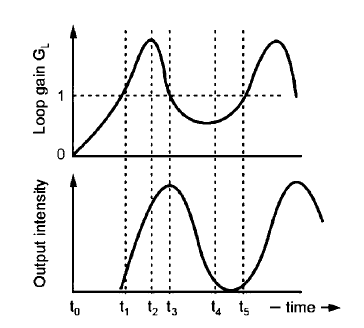
\includegraphics[width=8cm]{pic1}
\end{center}
\par  
3. How Q-Swith mode of our Nd:YAG laser is implemented with the help of scheme below?
\begin{center}
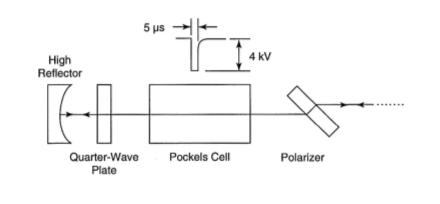
\includegraphics[width=10cm]{pic2}
\end{center}
As shown in the figure above, when 0 voltage of Pockel Cell and laser comes from left to Quarter-wave plate, the linear polarization light changes from horizontal to vertical by passing the Quarter-wave plate twice. So the beam can not transmit polarizer slit and keep accumulating in the resonator. When the Pockel Cell is charged to certain voltage that exactly compensates the polarization of Quarter-wave plate, the beam then travel passes the Polarizer slit, and a intense pulse outputs. \\
\par 
4. How is mode-selection perfermed in this laser?\par 
In this laser, longitudinal mode was selected by nonlinear crystal with Kerr effect. Kerr effect only helps to focus high intense light and eventually a single giant pulse outputs after many times' travel in the resonator. \\
\par 
5. Why are the pump chambers of the amplifier outside the oscillator resonator? What would happen if they were inside the oscillator?\par 
It helps to generate short time and uniform pulse. In the resonator, the incident beam travel back and forth for many times. If pump chambers were put inside the resonator, when beam travel across the crystal, different frequencys go with different time duration, thus it would strench the width of beam and eventually elongate the time duration of laser. And polarization dispersion would happen as well.\\
\par 
\section{Brief Report}
In this demonstration, we first go through each component of this ns-Laser Flash Photolysis system. This laser system is to generate laser pulse in ns scale duration


\end{document}
